\documentclass[12pt]{amsart}

\theoremstyle{plain}
\newtheorem{theorem}{Theorem}
\newtheorem{lemma}[theorem]{Lemma} 
\newtheorem{conjecture}[theorem]{Conjecture} 
\newtheorem{corollary}[theorem]{Corollary}
\newtheorem{proposition}[theorem]{Proposition}
\theoremstyle{definition}
\newtheorem{definition}[theorem]{Definition}
\newtheorem*{question}{Question}

\usepackage{fullpage,hyperref,url}
\usepackage[pdftex]{graphicx}
\usepackage{lscape}

\title{Quintic Spectrahedra}
\author{Jacob Emmert-Aronson}
\author{Moor Xu}
\date{May 7, 2014}
\begin{document} 
\maketitle

\section{Background}

\emph{Spectrahedra} of degree $n$ in $\mathbb{R}^k$ are convex bodies
given by $k$-dimensional affine slices of the cone of $n \times n$
positive semidefinite matrices.  They arise as feasible domains in
semidefinite programming and each is described by a linear matrix
inequality. We will work with spectrahedra in $\mathbb R^3$.

\begin{definition} 
	A \emph{spectrahedron} of degree $n$ in $\mathbb R^3$ is a convex body
	of the form 
	\[ 
		S = \left\{
		(x,y,z) \mid Ax + By + Cz + D \text{ is positive semidefinite} \right\}
	\] 
	where $A$, $B$, $C$, $D$ are real symmetric $n\times n$ matrices.
\end{definition} 

\bigskip
%\vspace\baselineskip

\begin{center}
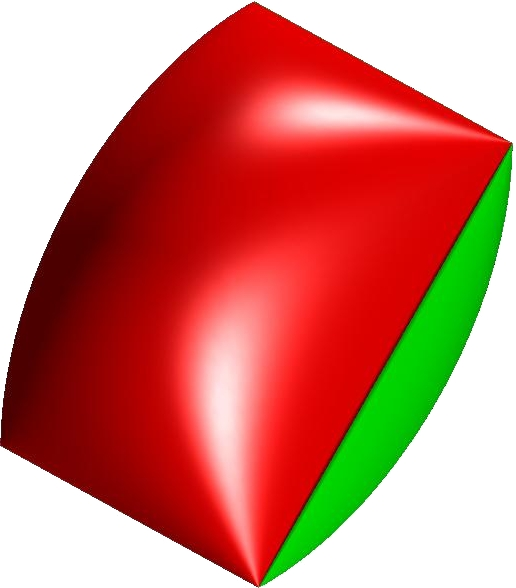
\includegraphics[scale=.15]{pillow.jpg}
%\vspace\baselineskip
\bigskip

{\small
\emph{The pillow}: the spectrahedron
$
\begin{pmatrix}
  1&x&0&x\\
  x&1&y&0\\
  0&y&1&z\\
  x&0&z&1
\end{pmatrix}
\succeq 0\text.$  Here $k=3,\, n=4$.}
\end{center}
%\vspace\baselineskip
\bigskip

Because the cost function of an SDP is linear, the optimal point
always lies on the surface.  One interesting and practically useful
question is the likelihood for the result of an optimization to be a
node, one of the corner points seen when visualizing the
spectrahedron.  A generic matrix represented by a point on the surface
of the spectrahedron has rank $n-1$, while the matrix at a node
typically has rank $n-2$.  This low-rank property of nodes often
translates to easier computation.

To better understand the nodal structure of spectrahedra, we work with the
notion of a symmetroid.
\begin{definition} 
	The \emph{symmetroid} $S$ of degree $n$ is a surface defined by 
	\[ 
		\det (Ax + By + Cz + D) = 0
	\] 
	where $A$, $B$, $C$, $D$ are $n\times n$ matrices.
\end{definition} 
A spectrahedron can be thought of as a component of the symmetroid.
To compute the nodes of a spectrahedron, we compute the nodes of the
symmetroid, and see how many lie on the spectrahedron.

\begin{proposition} 
	Generically, a symmetroid $S$ of degree $n$ has $\binom{n+1}3$ nodes.
\end{proposition} 

\begin{question} 
How many nodes can be real? How many nodes can lie on the spectrahedron?
\end{question} 

These questions have been answered in the quartic case. 
\cite{OKSV} classifies the number of nodes that quartic spectrahedra can have. 
\begin{theorem}\label{quartic}
	There exists a quartic spectrahedron with $\sigma$ nodes on its boundary and
	$\rho$ real nodes in its symmetroid if and only if $0 \le \sigma \le \rho$,
	both are even, and $2 \le \rho \le 10$.
\end{theorem} 
Hence there are 20 types of quartic spectrahedra, each with its own
$(\rho, \sigma)$ node count. 

\section{The Quintic Case}

We studied the nodal structure of quintic spectrahedra in hopes of obtaining an
analogous result.

To carry this out, we generated random spectrahedra and computed
the positions of nodes, while also running multiple optimization
problems on each.  Jacob Emmert-Aronson and Joe Kileel wrote much of
the code to carry this out last semester.  
We had used Singular
to determine locations of nodes through a Gr\"obner basis algorithm;
due to apparent numeric instabilities, however, this misidentified
nodes in certain edge cases.  We have replaced this with the
homotopy algorithms implemented in Bertini, which have produced more
reliable results.  

More specifically, here is what we did:
\begin{itemize}
	\item Generate matrices $A$, $B$, $C$, $D$.
	\item Use Bertini to compute the 20 complex nodes.
	\item Count the number of real nodes.
	\item For each real node, check if it lies on the spectrahedron. (A node
		lies on the spectrahedron if its eigenvalues have the same sign.)
\end{itemize}

Initially, we generated matrices $A$, $B$, $C$ by selecting their entries from
a Gaussian distribution with mean 0 and standard deviation 1000, and choosing
$D$ as the identity matrix. This meant that our spectrahedra always contained
the origin. This method of sampling, however, did not allow us to find
spectrahedra with high numbers of nodes. Since then, we have used different
sampling methods as well. For example, we can force nodes at $(0,0,0)$,
$(1,0,0)$, $(0,1,0)$, and $(0,0,1)$ in order to skew the distribution of
spectrahedra toward those with higher node counts.

So far, after generating more than 10000 random quintic spectrahedra, we have
observed 45 types of spectrahedra. 
We conjecture that a result analogous to Theorem \ref{quartic} holds in the
quintic case, which would suggest that there should be 65 different types of
quintic spectrahedra.
\begin{conjecture} 
	There exists a quintic spectrahedron with $\sigma$ nodes on its boundary and
	$\rho$ real nodes in its symmetroid if and only if $0 \le \sigma \le \rho$,
	both are even, and $2 \le \rho \le 20$.
\end{conjecture} 

\section{Gallery of Spectrahedra}

We have so far seen 45 types of spectrahedra out of the 65 types that are
conjectured to exist. The missing types are all spectrahedra with 
at least $12$ spectrahedral nodes, spectrahedra with $0$ spectrahedral nodes
and $\ge 12$ symmetroid nodes, as well as types 
$(\rho,\sigma) = (8,8), (10,10), (12,12), (18,2), (20,2)$.
We believe that these types are missing because they are rare, but examples do
exist and can be found.

\bigskip

\begin{center}
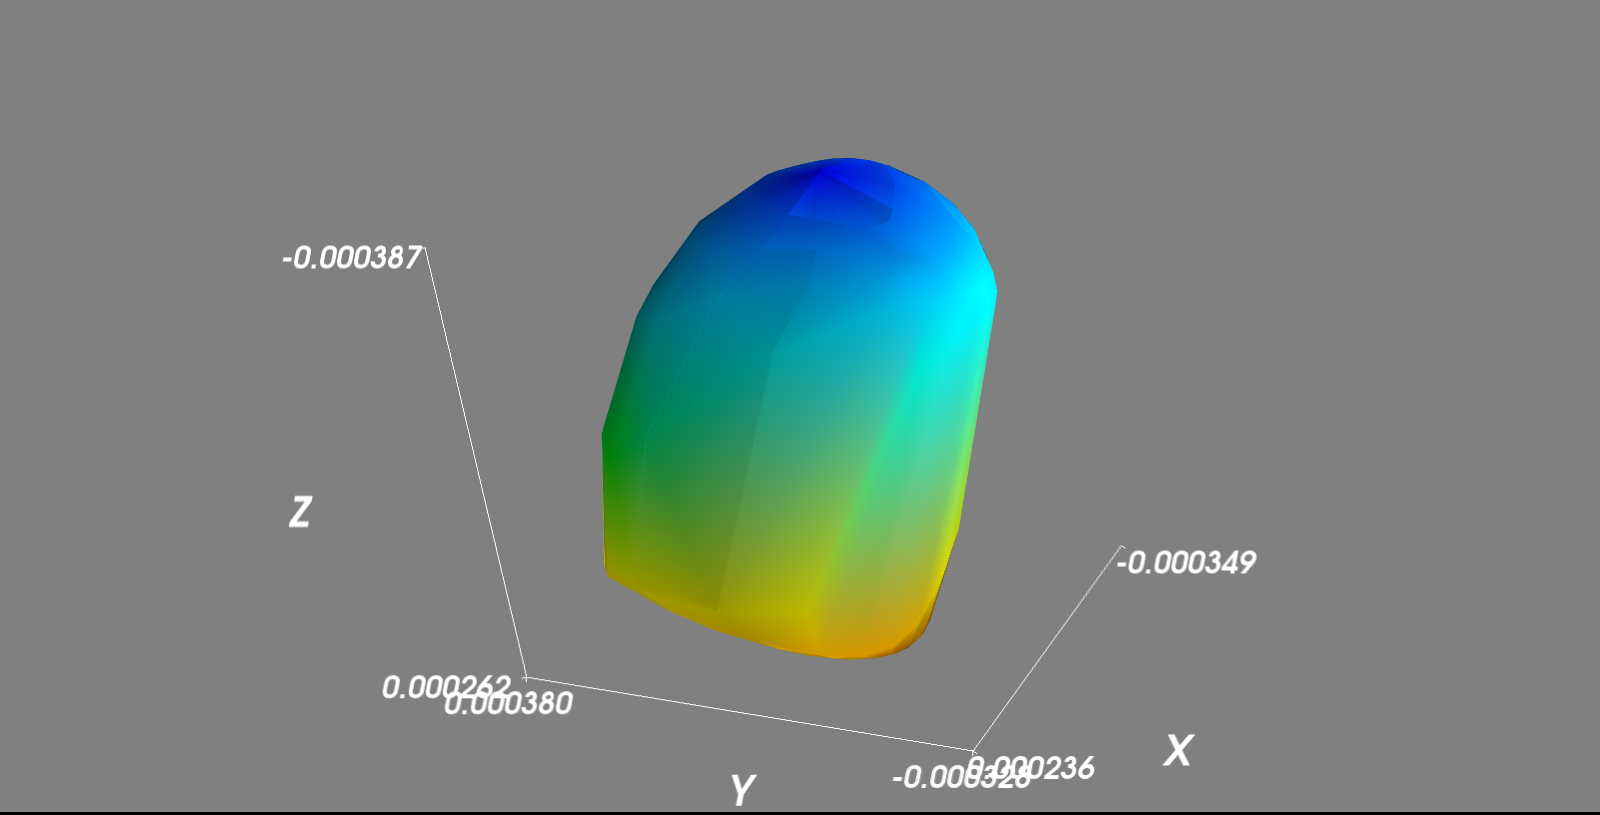
\includegraphics[height=1.8in]{0200}

{\small A spectrahedron of type $(\rho,\sigma) = (2,0)$.}
\end{center}

\bigskip

\begin{center}
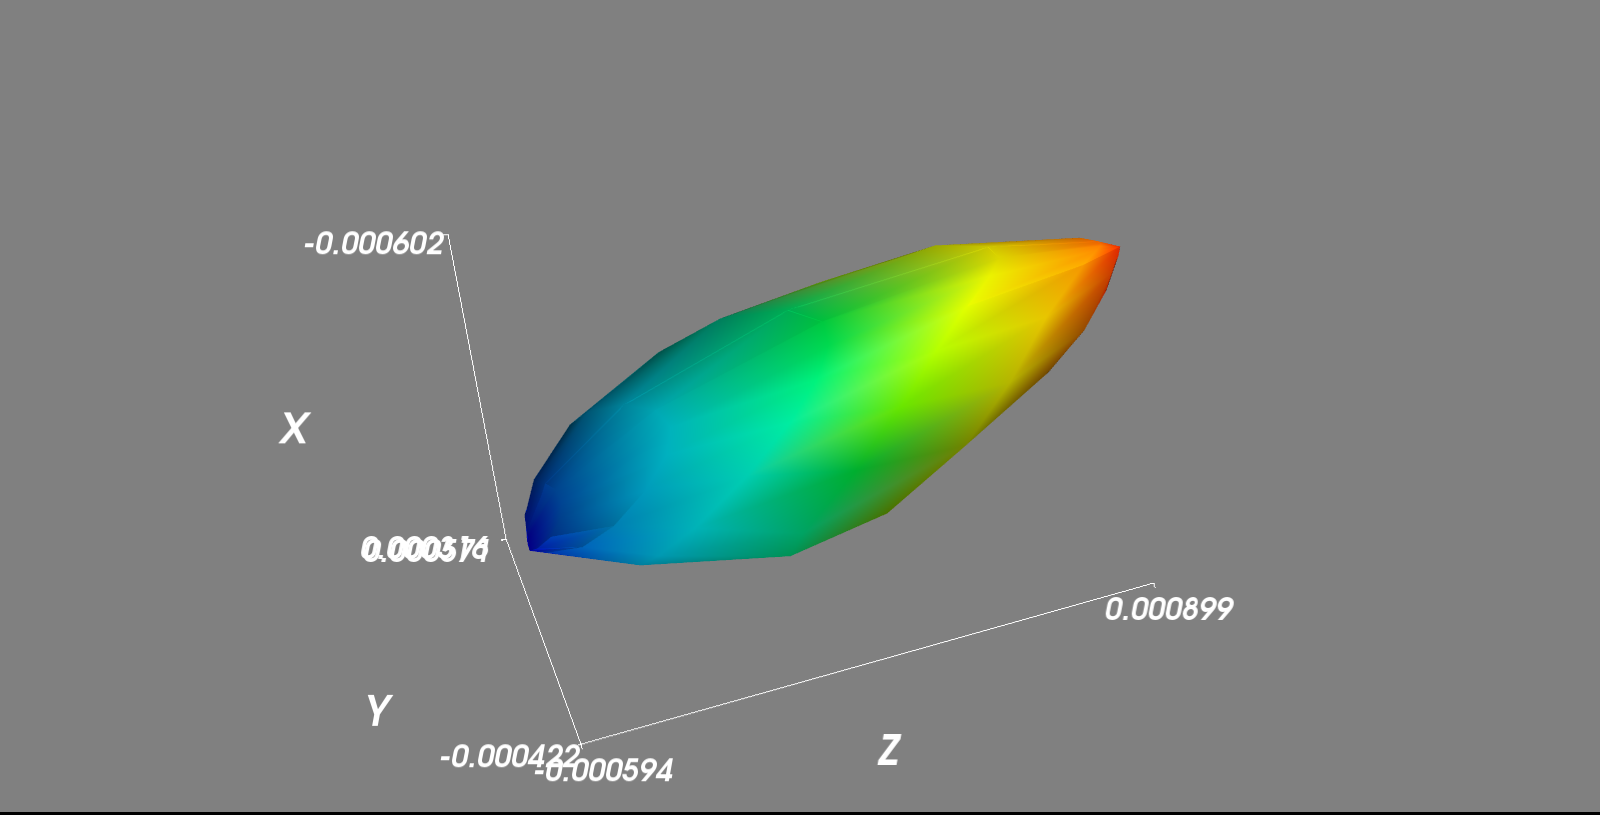
\includegraphics[height=1.8in]{0202}

{\small A spectrahedron of type $(\rho,\sigma) = (2,2)$.}
\end{center}

\bigskip

\begin{center}
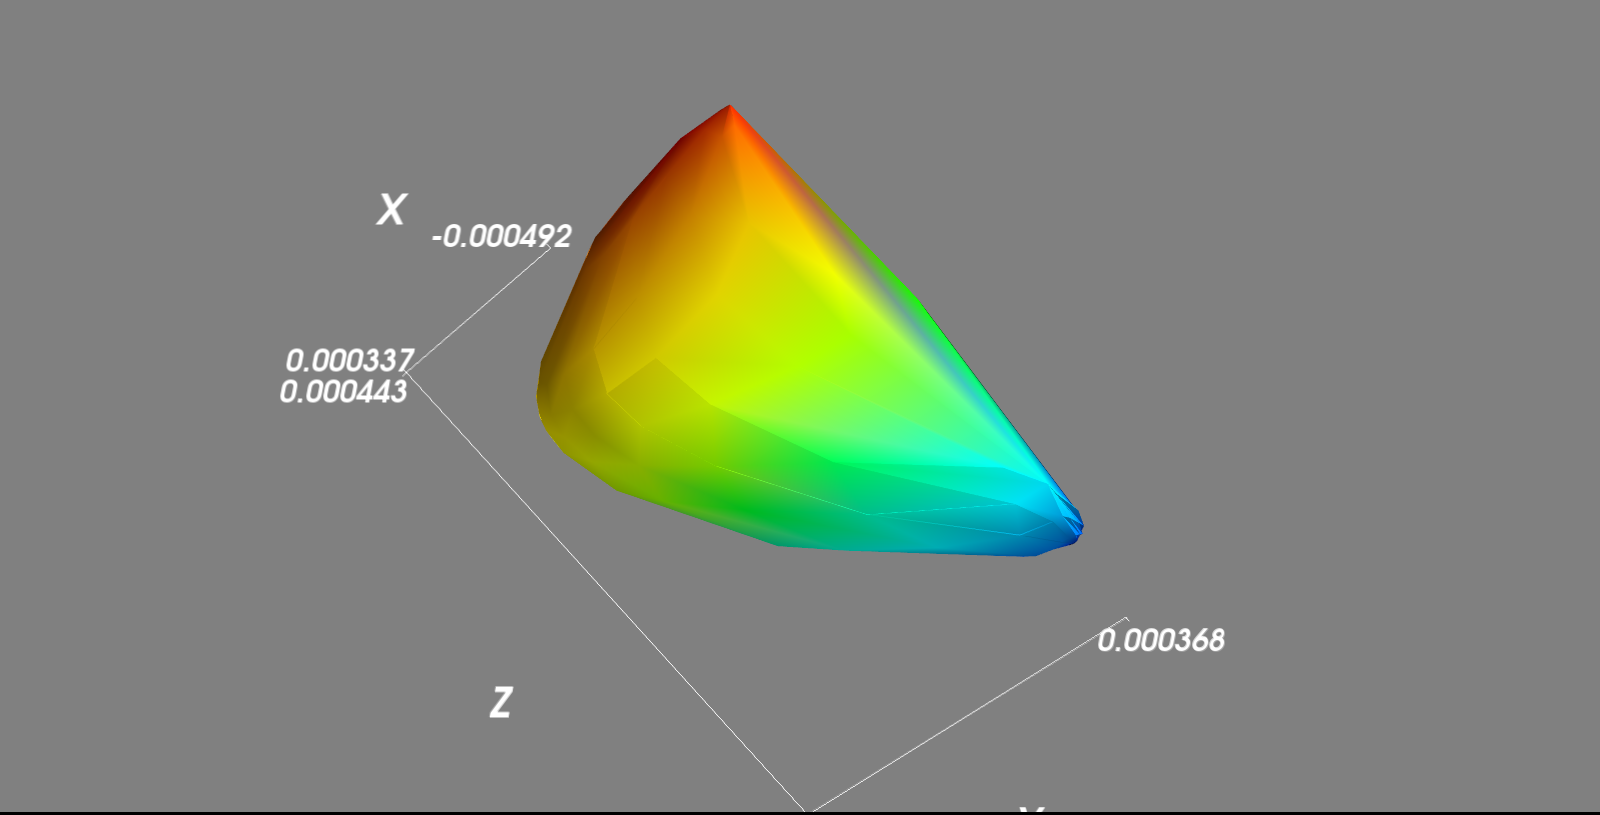
\includegraphics[height=1.8in]{0404}

{\small A spectrahedron of type $(\rho,\sigma) = (4,4)$.}
\end{center}

\bigskip







On the following pages, we provide an example of a spectrahedron from each of
the 45 types that we have found so far, giving a zoo of spectrahedra.

\begin{landscape}
\thispagestyle{empty}
\tiny
\begin{align*} 
(2,0) &:
\begin{bmatrix}
3138  &   -1780  &   822  &   -125  &   771  \\ 
 -1780  &   -945  &   -1275  &   359  &   -367  \\ 
 822  &   -1275  &   -1980  &   -1422  &   1094  \\ 
 -125  &   359  &   -1422  &   -1088  &   1650  \\ 
 771  &   -367  &   1094  &   1650  &   -1740  \\ 
\end{bmatrix}
\begin{bmatrix}
941  &   -1943  &   599  &   1951  &   18  \\ 
 -1943  &   460  &   -1662  &   920  &   830  \\ 
 599  &   -1662  &   671  &   723  &   215  \\ 
 1951  &   920  &   723  &   1004  &   165  \\ 
 18  &   830  &   215  &   165  &   -1574  \\ 
\end{bmatrix}
\begin{bmatrix}
-1590  &   345  &   49  &   -443  &   1136  \\ 
 345  &   -1102  &   -364  &   -212  &   -936  \\ 
 49  &   -364  &   181  &   -1124  &   -2491  \\ 
 -443  &   -212  &   -1124  &   860  &   370  \\ 
 1136  &   -936  &   -2491  &   370  &   -1570  \\ 
\end{bmatrix}
\begin{bmatrix}
1  &   0  &   0  &   0  &   0  \\ 
 0  &   1  &   0  &   0  &   0  \\ 
 0  &   0  &   1  &   0  &   0  \\ 
 0  &   0  &   0  &   1  &   0  \\ 
 0  &   0  &   0  &   0  &   1  \\ 
\end{bmatrix} \\
(2,2) &:
\begin{bmatrix}
-1555  &   110  &   92  &   -694  &   28  \\ 
 110  &   -1188  &   95  &   -861  &   12  \\ 
 92  &   95  &   -212  &   965  &   -2797  \\ 
 -694  &   -861  &   965  &   -1206  &   1125  \\ 
 28  &   12  &   -2797  &   1125  &   -1279  \\ 
\end{bmatrix}
\begin{bmatrix}
599  &   -905  &   -944  &   370  &   -365  \\ 
 -905  &   -168  &   612  &   -273  &   -373  \\ 
 -944  &   612  &   1785  &   -894  &   1426  \\ 
 370  &   -273  &   -894  &   1536  &   464  \\ 
 -365  &   -373  &   1426  &   464  &   -760  \\ 
\end{bmatrix}
\begin{bmatrix}
195  &   -62  &   -755  &   -349  &   962  \\ 
 -62  &   -337  &   -963  &   549  &   -1033  \\ 
 -755  &   -963  &   467  &   -556  &   -323  \\ 
 -349  &   549  &   -556  &   -573  &   -32  \\ 
 962  &   -1033  &   -323  &   -32  &   247  \\ 
\end{bmatrix}
\begin{bmatrix}
1  &   0  &   0  &   0  &   0  \\ 
 0  &   1  &   0  &   0  &   0  \\ 
 0  &   0  &   1  &   0  &   0  \\ 
 0  &   0  &   0  &   1  &   0  \\ 
 0  &   0  &   0  &   0  &   1  \\ 
\end{bmatrix}
\\
(4,0) &:
\begin{bmatrix}
1206  &   -258  &   -198  &   1068  &   126  \\ 
 -258  &   557  &   -1820  &   -1297  &   42  \\ 
 -198  &   -1820  &   1638  &   1244  &   851  \\ 
 1068  &   -1297  &   1244  &   561  &   444  \\ 
 126  &   42  &   851  &   444  &   -1551  \\ 
\end{bmatrix}
\begin{bmatrix}
-178  &   421  &   -13  &   883  &   -464  \\ 
 421  &   -1359  &   2074  &   2909  &   -334  \\ 
 -13  &   2074  &   -1037  &   -692  &   -415  \\ 
 883  &   2909  &   -692  &   1575  &   -824  \\ 
 -464  &   -334  &   -415  &   -824  &   -653  \\ 
\end{bmatrix}
\begin{bmatrix}
1537  &   -369  &   -750  &   -2516  &   82  \\ 
 -369  &   139  &   -229  &   -1371  &   92  \\ 
 -750  &   -229  &   -459  &   -321  &   365  \\ 
 -2516  &   -1371  &   -321  &   784  &   -314  \\ 
 82  &   92  &   365  &   -314  &   874  \\ 
\end{bmatrix}
\begin{bmatrix}
1  &   0  &   0  &   0  &   0  \\ 
 0  &   1  &   0  &   0  &   0  \\ 
 0  &   0  &   1  &   0  &   0  \\ 
 0  &   0  &   0  &   1  &   0  \\ 
 0  &   0  &   0  &   0  &   1  \\ 
\end{bmatrix}
\\
(4,2) &:
\begin{bmatrix}
-439  &   739  &   780  &   -1661  &   -1304  \\ 
 739  &   -1740  &   -433  &   100  &   268  \\ 
 780  &   -433  &   -54  &   -49  &   370  \\ 
 -1661  &   100  &   -49  &   1197  &   -590  \\ 
 -1304  &   268  &   370  &   -590  &   263  \\ 
\end{bmatrix}
\begin{bmatrix}
-1986  &   -628  &   1085  &   -1063  &   541  \\ 
 -628  &   287  &   -1556  &   1466  &   -715  \\ 
 1085  &   -1556  &   -270  &   -178  &   -942  \\ 
 -1063  &   1466  &   -178  &   -1528  &   1253  \\ 
 541  &   -715  &   -942  &   1253  &   -183  \\ 
\end{bmatrix}
\begin{bmatrix}
-852  &   -218  &   -633  &   958  &   796  \\ 
 -218  &   823  &   -610  &   -1635  &   -1478  \\ 
 -633  &   -610  &   -8  &   -1672  &   -1336  \\ 
 958  &   -1635  &   -1672  &   -492  &   -15  \\ 
 796  &   -1478  &   -1336  &   -15  &   -490  \\ 
\end{bmatrix}
\begin{bmatrix}
1  &   0  &   0  &   0  &   0  \\ 
 0  &   1  &   0  &   0  &   0  \\ 
 0  &   0  &   1  &   0  &   0  \\ 
 0  &   0  &   0  &   1  &   0  \\ 
 0  &   0  &   0  &   0  &   1  \\ 
\end{bmatrix}
\\
(4,4) &:
\begin{bmatrix}
758  &   125  &   -1476  &   -291  &   -4  \\ 
 125  &   -192  &   -231  &   229  &   1080  \\ 
 -1476  &   -231  &   375  &   767  &   -855  \\ 
 -291  &   229  &   767  &   -68  &   1068  \\ 
 -4  &   1080  &   -855  &   1068  &   -1834  \\ 
\end{bmatrix}
\begin{bmatrix}
-388  &   -1353  &   -578  &   -314  &   -912  \\ 
 -1353  &   -2163  &   -869  &   -193  &   60  \\ 
 -578  &   -869  &   2664  &   -910  &   1022  \\ 
 -314  &   -193  &   -910  &   1110  &   1171  \\ 
 -912  &   60  &   1022  &   1171  &   -852  \\ 
\end{bmatrix}
\begin{bmatrix}
436  &   241  &   372  &   -1118  &   -485  \\ 
 241  &   -831  &   -1076  &   872  &   566  \\ 
 372  &   -1076  &   709  &   -781  &   -69  \\ 
 -1118  &   872  &   -781  &   239  &   -903  \\ 
 -485  &   566  &   -69  &   -903  &   -1500  \\ 
\end{bmatrix}
\begin{bmatrix}
1  &   0  &   0  &   0  &   0  \\ 
 0  &   1  &   0  &   0  &   0  \\ 
 0  &   0  &   1  &   0  &   0  \\ 
 0  &   0  &   0  &   1  &   0  \\ 
 0  &   0  &   0  &   0  &   1  \\ 
\end{bmatrix}
\\
(6,0) &:
\begin{bmatrix}
1158  &   1110  &   530  &   -359  &   92  \\ 
 1110  &   -1380  &   -1690  &   330  &   -310  \\ 
 530  &   -1690  &   225  &   -1336  &   -990  \\ 
 -359  &   330  &   -1336  &   -186  &   251  \\ 
 92  &   -310  &   -990  &   251  &   194  \\ 
\end{bmatrix}
\begin{bmatrix}
268  &   -1104  &   -588  &   693  &   290  \\ 
 -1104  &   -1367  &   76  &   230  &   -1433  \\ 
 -588  &   76  &   341  &   2026  &   -828  \\ 
 693  &   230  &   2026  &   550  &   -419  \\ 
 290  &   -1433  &   -828  &   -419  &   535  \\ 
\end{bmatrix}
\begin{bmatrix}
122  &   -431  &   -1557  &   -1047  &   -138  \\ 
 -431  &   -1618  &   -677  &   383  &   -173  \\ 
 -1557  &   -677  &   71  &   143  &   417  \\ 
 -1047  &   383  &   143  &   -194  &   -280  \\ 
 -138  &   -173  &   417  &   -280  &   633  \\ 
\end{bmatrix}
\begin{bmatrix}
1  &   0  &   0  &   0  &   0  \\ 
 0  &   1  &   0  &   0  &   0  \\ 
 0  &   0  &   1  &   0  &   0  \\ 
 0  &   0  &   0  &   1  &   0  \\ 
 0  &   0  &   0  &   0  &   1  \\ 
\end{bmatrix}
\\
(6,2) &:
\begin{bmatrix}
107  &   -2070  &   3772  &   3183  &   -877  \\ 
 -2070  &   8089  &   -4303  &   -7235  &   -618  \\ 
 3772  &   -4303  &   4198  &   3116  &   -1287  \\ 
 3183  &   -7235  &   3116  &   14047  &   -7863  \\ 
 -877  &   -618  &   -1287  &   -7863  &   2329  \\ 
\end{bmatrix}
\begin{bmatrix}
-4277  &   -2710  &   3327  &   4344  &   -1832  \\ 
 -2710  &   8849  &   -5303  &   -8703  &   2139  \\ 
 3327  &   -5303  &   3071  &   -101  &   1030  \\ 
 4344  &   -8703  &   -101  &   7592  &   -3534  \\ 
 -1832  &   2139  &   1030  &   -3534  &   1857  \\ 
\end{bmatrix}
\begin{bmatrix}
-1447  &   -2171  &   2877  &   3036  &   421  \\ 
 -2171  &   5216  &   -5624  &   -9508  &   3094  \\ 
 2877  &   -5624  &   3276  &   1240  &   412  \\ 
 3036  &   -9508  &   1240  &   9665  &   -3864  \\ 
 421  &   3094  &   412  &   -3864  &   1092  \\ 
\end{bmatrix}
\begin{bmatrix}
-1259  &   3134  &   -1777  &   -2214  &   242  \\ 
 3134  &   -8458  &   4713  &   7395  &   -1530  \\ 
 -1777  &   4713  &   -3821  &   -1799  &   -375  \\ 
 -2214  &   7395  &   -1799  &   -13222  &   5135  \\ 
 242  &   -1530  &   -375  &   5135  &   -2426  \\ 
\end{bmatrix}
\\
(6,4) &:
\begin{bmatrix}
3597  &   1738  &   854  &   -1886  &   1556  \\ 
 1738  &   402  &   -948  &   324  &   1760  \\ 
 854  &   -948  &   -2145  &   3135  &   -742  \\ 
 -1886  &   324  &   3135  &   -4210  &   -821  \\ 
 1556  &   1760  &   -742  &   -821  &   3812  \\ 
\end{bmatrix}
\begin{bmatrix}
2495  &   1730  &   -1151  &   -1015  &   -1530  \\ 
 1730  &   369  &   -1423  &   -1470  &   3383  \\ 
 -1151  &   -1423  &   -1920  &   422  &   880  \\ 
 -1015  &   -1470  &   422  &   2284  &   2023  \\ 
 -1530  &   3383  &   880  &   2023  &   1802  \\ 
\end{bmatrix}
\begin{bmatrix}
-3840  &   -96  &   -2344  &   1220  &   -900  \\ 
 -96  &   -503  &   1121  &   -519  &   871  \\ 
 -2344  &   1121  &   -3153  &   269  &   -1225  \\ 
 1220  &   -519  &   269  &   -4757  &   1171  \\ 
 -900  &   871  &   -1225  &   1171  &   3984  \\ 
\end{bmatrix}
\begin{bmatrix}
-4000  &   -1740  &   -156  &   744  &   -1348  \\ 
 -1740  &   -1494  &   270  &   1296  &   -1110  \\ 
 -156  &   270  &   -161  &   -414  &   202  \\ 
 744  &   1296  &   -414  &   -1556  &   208  \\ 
 -1348  &   -1110  &   202  &   208  &   -4814  \\ 
\end{bmatrix}
\\
\end{align*} 
\end{landscape}

\begin{landscape}
\thispagestyle{empty}
\tiny
\begin{align*} 
(6,6) &:
\begin{bmatrix}
-549  &   -1017  &   858  &   486  &   215  \\ 
 -1017  &   3223  &   -2873  &   -786  &   -3829  \\ 
 858  &   -2873  &   1289  &   2072  &   158  \\ 
 486  &   -786  &   2072  &   -831  &   2820  \\ 
 215  &   -3829  &   158  &   2820  &   2130  \\ 
\end{bmatrix}
\begin{bmatrix}
-1935  &   -4601  &   292  &   -425  &   -1777  \\ 
 -4601  &   -3985  &   -386  &   -450  &   -4875  \\ 
 292  &   -386  &   -422  &   -1221  &   736  \\ 
 -425  &   -450  &   -1221  &   -2488  &   -170  \\ 
 -1777  &   -4875  &   736  &   -170  &   3128  \\ 
\end{bmatrix}
\begin{bmatrix}
-757  &   -2828  &   1833  &   1509  &   580  \\ 
 -2828  &   802  &   -630  &   -1442  &   -1937  \\ 
 1833  &   -630  &   224  &   356  &   619  \\ 
 1509  &   -1442  &   356  &   162  &   336  \\ 
 580  &   -1937  &   619  &   336  &   4057  \\ 
\end{bmatrix}
\begin{bmatrix}
-542  &   1158  &   -478  &   -733  &   98  \\ 
 1158  &   -4276  &   2006  &   2124  &   2614  \\ 
 -478  &   2006  &   -2123  &   -824  &   -1417  \\ 
 -733  &   2124  &   -824  &   -1178  &   -746  \\ 
 98  &   2614  &   -1417  &   -746  &   -4443  \\ 
\end{bmatrix}
\\
(8,0) &:
\begin{bmatrix}
1097  &   1705  &   642  &   -1217  &   -850  \\ 
 1705  &   551  &   -293  &   601  &   666  \\ 
 642  &   -293  &   29  &   -317  &   896  \\ 
 -1217  &   601  &   -317  &   -121  &   -1328  \\ 
 -850  &   666  &   896  &   -1328  &   429  \\ 
\end{bmatrix}
\begin{bmatrix}
1333  &   665  &   -682  &   -28  &   1177  \\ 
 665  &   -372  &   2  &   -347  &   -1291  \\ 
 -682  &   2  &   47  &   181  &   695  \\ 
 -28  &   -347  &   181  &   100  &   232  \\ 
 1177  &   -1291  &   695  &   232  &   -541  \\ 
\end{bmatrix}
\begin{bmatrix}
-1280  &   323  &   -945  &   748  &   -350  \\ 
 323  &   553  &   161  &   1121  &   -849  \\ 
 -945  &   161  &   -1109  &   -748  &   1643  \\ 
 748  &   1121  &   -748  &   -934  &   1774  \\ 
 -350  &   -849  &   1643  &   1774  &   -2608  \\ 
\end{bmatrix}
\begin{bmatrix}
1  &   0  &   0  &   0  &   0  \\ 
 0  &   1  &   0  &   0  &   0  \\ 
 0  &   0  &   1  &   0  &   0  \\ 
 0  &   0  &   0  &   1  &   0  \\ 
 0  &   0  &   0  &   0  &   1  \\ 
\end{bmatrix}
\\
(8,2) &:
\begin{bmatrix}
-472  &   3370  &   -2386  &   -2378  &   -2682  \\ 
 3370  &   3520  &   -1998  &   3841  &   -2020  \\ 
 -2386  &   -1998  &   972  &   -913  &   -3227  \\ 
 -2378  &   3841  &   -913  &   -9088  &   2395  \\ 
 -2682  &   -2020  &   -3227  &   2395  &   -5612  \\ 
\end{bmatrix}
\begin{bmatrix}
-649  &   -12  &   446  &   -1229  &   -493  \\ 
 -12  &   -1400  &   -901  &   2861  &   -3359  \\ 
 446  &   -901  &   520  &   83  &   -830  \\ 
 -1229  &   2861  &   83  &   -7865  &   4994  \\ 
 -493  &   -3359  &   -830  &   4994  &   -3740  \\ 
\end{bmatrix}
\begin{bmatrix}
-8625  &   3318  &   1654  &   -2983  &   -4347  \\ 
 3318  &   -990  &   40  &   4904  &   -1351  \\ 
 1654  &   40  &   -6552  &   -95  &   1573  \\ 
 -2983  &   4904  &   -95  &   -11363  &   3023  \\ 
 -4347  &   -1351  &   1573  &   3023  &   -5016  \\ 
\end{bmatrix}
\begin{bmatrix}
409  &   -530  &   -62  &   861  &   -825  \\ 
 -530  &   -644  &   424  &   -3033  &   2811  \\ 
 -62  &   424  &   148  &   -1131  &   381  \\ 
 861  &   -3033  &   -1131  &   8889  &   -3870  \\ 
 -825  &   2811  &   381  &   -3870  &   1575  \\ 
\end{bmatrix}
\\
(8,4) &:
\begin{bmatrix}
1333  &   1964  &   -2304  &   587  &   -3145  \\ 
 1964  &   697  &   183  &   500  &   -1822  \\ 
 -2304  &   183  &   -1159  &   1120  &   1126  \\ 
 587  &   500  &   1120  &   4565  &   1205  \\ 
 -3145  &   -1822  &   1126  &   1205  &   3273  \\ 
\end{bmatrix}
\begin{bmatrix}
2001  &   212  &   -1246  &   -1825  &   -2831  \\ 
 212  &   -581  &   141  &   1958  &   -1968  \\ 
 -1246  &   141  &   -804  &   -2569  &   2508  \\ 
 -1825  &   1958  &   -2569  &   -239  &   3502  \\ 
 -2831  &   -1968  &   2508  &   3502  &   4238  \\ 
\end{bmatrix}
\begin{bmatrix}
-2749  &   479  &   -2744  &   -1803  &   -2498  \\ 
 479  &   184  &   -2059  &   878  &   334  \\ 
 -2744  &   -2059  &   -3994  &   -4097  &   -364  \\ 
 -1803  &   878  &   -4097  &   2181  &   -1963  \\ 
 -2498  &   334  &   -364  &   -1963  &   -4388  \\ 
\end{bmatrix}
\begin{bmatrix}
-3901  &   -1036  &   722  &   1015  &   3637  \\ 
 -1036  &   -1341  &   853  &   -1356  &   1794  \\ 
 722  &   853  &   -650  &   249  &   -1524  \\ 
 1015  &   -1356  &   249  &   -5822  &   -1499  \\ 
 3637  &   1794  &   -1524  &   -1499  &   -5105  \\ 
\end{bmatrix}
\\
(8,6) &:
\begin{bmatrix}
1112  &   -4233  &   7  &   1091  &   736  \\ 
 -4233  &   -3813  &   -1522  &   2847  &   576  \\ 
 7  &   -1522  &   2395  &   -2275  &   -109  \\ 
 1091  &   2847  &   -2275  &   6570  &   -188  \\ 
 736  &   576  &   -109  &   -188  &   -176  \\ 
\end{bmatrix}
\begin{bmatrix}
-5926  &   -4140  &   896  &   -2563  &   -101  \\ 
 -4140  &   -1714  &   -3920  &   409  &   -48  \\ 
 896  &   -3920  &   1496  &   -716  &   -178  \\ 
 -2563  &   409  &   -716  &   6679  &   -711  \\ 
 -101  &   -48  &   -178  &   -711  &   168  \\ 
\end{bmatrix}
\begin{bmatrix}
-2182  &   -3668  &   2678  &   3867  &   -2695  \\ 
 -3668  &   -285  &   -1689  &   -1653  &   -2816  \\ 
 2678  &   -1689  &   651  &   -4505  &   730  \\ 
 3867  &   -1653  &   -4505  &   2991  &   2423  \\ 
 -2695  &   -2816  &   730  &   2423  &   -2799  \\ 
\end{bmatrix}
\begin{bmatrix}
-1522  &   2446  &   40  &   -573  &   -545  \\ 
 2446  &   -4472  &   1340  &   48  &   516  \\ 
 40  &   1340  &   -3652  &   2076  &   974  \\ 
 -573  &   48  &   2076  &   -8469  &   72  \\ 
 -545  &   516  &   974  &   72  &   -542  \\ 
\end{bmatrix}
\\
(10,0) &:
\begin{bmatrix}
913  &   -908  &   519  &   -223  &   30  \\ 
 -908  &   811  &   -106  &   426  &   -937  \\ 
 519  &   -106  &   -495  &   -291  &   -2011  \\ 
 -223  &   426  &   -291  &   421  &   -684  \\ 
 30  &   -937  &   -2011  &   -684  &   -1149  \\ 
\end{bmatrix}
\begin{bmatrix}
926  &   542  &   -257  &   -1320  &   -32  \\ 
 542  &   568  &   624  &   -1797  &   -420  \\ 
 -257  &   624  &   668  &   639  &   -1142  \\ 
 -1320  &   -1797  &   639  &   712  &   -602  \\ 
 -32  &   -420  &   -1142  &   -602  &   -187  \\ 
\end{bmatrix}
\begin{bmatrix}
1940  &   -1206  &   671  &   142  &   -669  \\ 
 -1206  &   235  &   -1443  &   419  &   48  \\ 
 671  &   -1443  &   -1159  &   -976  &   -170  \\ 
 142  &   419  &   -976  &   71  &   141  \\ 
 -669  &   48  &   -170  &   141  &   -1083  \\ 
\end{bmatrix}
\begin{bmatrix}
1  &   0  &   0  &   0  &   0  \\ 
 0  &   1  &   0  &   0  &   0  \\ 
 0  &   0  &   1  &   0  &   0  \\ 
 0  &   0  &   0  &   1  &   0  \\ 
 0  &   0  &   0  &   0  &   1  \\ 
\end{bmatrix}
\\
(10,2) &:
\begin{bmatrix}
-2817  &   554  &   -346  &   611  &   -2446  \\ 
 554  &   1468  &   49  &   444  &   -1422  \\ 
 -346  &   49  &   226  &   -774  &   -2352  \\ 
 611  &   444  &   -774  &   -537  &   1155  \\ 
 -2446  &   -1422  &   -2352  &   1155  &   -6855  \\ 
\end{bmatrix}
\begin{bmatrix}
-1168  &   -2331  &   -610  &   -3375  &   -2196  \\ 
 -2331  &   -3602  &   1365  &   -1269  &   -1941  \\ 
 -610  &   1365  &   2773  &   2195  &   1640  \\ 
 -3375  &   -1269  &   2195  &   5047  &   2251  \\ 
 -2196  &   -1941  &   1640  &   2251  &   -1238  \\ 
\end{bmatrix}
\begin{bmatrix}
-408  &   -256  &   -1751  &   -83  &   283  \\ 
 -256  &   908  &   -698  &   1058  &   -1856  \\ 
 -1751  &   -698  &   -3348  &   -1866  &   -1251  \\ 
 -83  &   1058  &   -1866  &   -2054  &   966  \\ 
 283  &   -1856  &   -1251  &   966  &   -4067  \\ 
\end{bmatrix}
\begin{bmatrix}
-32  &   -174  &   379  &   1  &   -179  \\ 
 -174  &   -1817  &   -690  &   -374  &   1102  \\ 
 379  &   -690  &   -1876  &   930  &   117  \\ 
 1  &   -374  &   930  &   240  &   -711  \\ 
 -179  &   1102  &   117  &   -711  &   534  \\ 
\end{bmatrix}
\\
(10,4) &:
\begin{bmatrix}
-450  &   5000  &   -1562  &   615  &   -1099  \\ 
 5000  &   402  &   -332  &   -3720  &   25  \\ 
 -1562  &   -332  &   158  &   3002  &   -216  \\ 
 615  &   -3720  &   3002  &   -5377  &   -2159  \\ 
 -1099  &   25  &   -216  &   -2159  &   -1635  \\ 
\end{bmatrix}
\begin{bmatrix}
2068  &   2525  &   -887  &   -2196  &   -946  \\ 
 2525  &   1653  &   -724  &   -2701  &   -2068  \\ 
 -887  &   -724  &   807  &   1500  &   186  \\ 
 -2196  &   -2701  &   1500  &   -2542  &   -2831  \\ 
 -946  &   -2068  &   186  &   -2831  &   -2885  \\ 
\end{bmatrix}
\begin{bmatrix}
2196  &   2357  &   -819  &   -2284  &   -417  \\ 
 2357  &   2203  &   -1076  &   -3197  &   -754  \\ 
 -819  &   -1076  &   858  &   1413  &   -377  \\ 
 -2284  &   -3197  &   1413  &   -3254  &   -2172  \\ 
 -417  &   -754  &   -377  &   -2172  &   -2025  \\ 
\end{bmatrix}
\begin{bmatrix}
-2545  &   -2768  &   836  &   1938  &   448  \\ 
 -2768  &   -2984  &   751  &   2447  &   787  \\ 
 836  &   751  &   -1404  &   -1646  &   66  \\ 
 1938  &   2447  &   -1646  &   2364  &   2512  \\ 
 448  &   787  &   66  &   2512  &   1376  \\ 
\end{bmatrix}
\\
\end{align*} 
\end{landscape}


\begin{landscape}
\thispagestyle{empty}
\tiny
\begin{align*} 
(10,6) &:
\begin{bmatrix}
-458  &   922  &   -1502  &   -181  &   2166  \\ 
 922  &   979  &   -1790  &   -1664  &   -3573  \\ 
 -1502  &   -1790  &   -1301  &   375  &   418  \\ 
 -181  &   -1664  &   375  &   -2773  &   -4658  \\ 
 2166  &   -3573  &   418  &   -4658  &   -10774  \\ 
\end{bmatrix}
\begin{bmatrix}
-3382  &   -100  &   -2355  &   115  &   65  \\ 
 -100  &   -3223  &   1151  &   3310  &   -2419  \\ 
 -2355  &   1151  &   87  &   -603  &   1758  \\ 
 115  &   3310  &   -603  &   -7784  &   -2311  \\ 
 65  &   -2419  &   1758  &   -2311  &   -5881  \\ 
\end{bmatrix}
\begin{bmatrix}
-1609  &   2794  &   1165  &   170  &   340  \\ 
 2794  &   -8412  &   -4206  &   -2121  &   -2424  \\ 
 1165  &   -4206  &   -2310  &   2017  &   2928  \\ 
 170  &   -2121  &   2017  &   -1949  &   -4341  \\ 
 340  &   -2424  &   2928  &   -4341  &   -4840  \\ 
\end{bmatrix}
\begin{bmatrix}
-304  &   -858  &   1527  &   -175  &   -1370  \\ 
 -858  &   -1405  &   837  &   1026  &   2339  \\ 
 1527  &   837  &   -1556  &   -2200  &   -1657  \\ 
 -175  &   1026  &   -2200  &   1395  &   3836  \\ 
 -1370  &   2339  &   -1657  &   3836  &   3827  \\ 
\end{bmatrix}
\\
(10,8) &:
\begin{bmatrix}
9803  &   -1770  &   1174  &   -537  &   1779  \\ 
 -1770  &   610  &   679  &   -635  &   -257  \\ 
 1174  &   679  &   -584  &   -3023  &   195  \\ 
 -537  &   -635  &   -3023  &   -4013  &   -1799  \\ 
 1779  &   -257  &   195  &   -1799  &   -1052  \\ 
\end{bmatrix}
\begin{bmatrix}
7501  &   -958  &   705  &   1920  &   3862  \\ 
 -958  &   291  &   15  &   -1316  &   -203  \\ 
 705  &   15  &   -3096  &   -2102  &   3357  \\ 
 1920  &   -1316  &   -2102  &   -3705  &   -3588  \\ 
 3862  &   -203  &   3357  &   -3588  &   -4040  \\ 
\end{bmatrix}
\begin{bmatrix}
8097  &   -2404  &   285  &   -1646  &   3890  \\ 
 -2404  &   -5574  &   -1249  &   -130  &   -954  \\ 
 285  &   -1249  &   624  &   -1466  &   2179  \\ 
 -1646  &   -130  &   -1466  &   168  &   1158  \\ 
 3890  &   -954  &   2179  &   1158  &   -3413  \\ 
\end{bmatrix}
\begin{bmatrix}
-9830  &   1791  &   -1207  &   675  &   -1929  \\ 
 1791  &   -725  &   -404  &   439  &   173  \\ 
 -1207  &   -404  &   -1505  &   1012  &   -1014  \\ 
 675  &   439  &   1012  &   -845  &   449  \\ 
 -1929  &   173  &   -1014  &   449  &   -1110  \\ 
\end{bmatrix}
\\
(12,2) &:
\begin{bmatrix}
-3258  &   -792  &   5442  &   344  &   1437  \\ 
 -792  &   -1888  &   509  &   -1967  &   -4488  \\ 
 5442  &   509  &   -4912  &   1536  &   4675  \\ 
 344  &   -1967  &   1536  &   2854  &   3178  \\ 
 1437  &   -4488  &   4675  &   3178  &   1652  \\ 
\end{bmatrix}
\begin{bmatrix}
1504  &   -660  &   -996  &   -696  &   -430  \\ 
 -660  &   423  &   -369  &   -565  &   -704  \\ 
 -996  &   -369  &   954  &   -163  &   725  \\ 
 -696  &   -565  &   -163  &   -1188  &   -236  \\ 
 -430  &   -704  &   725  &   -236  &   -1370  \\ 
\end{bmatrix}
\begin{bmatrix}
-1341  &   -539  &   -841  &   -2201  &   154  \\ 
 -539  &   -970  &   -920  &   -2023  &   1313  \\ 
 -841  &   -920  &   592  &   -695  &   598  \\ 
 -2201  &   -2023  &   -695  &   -2218  &   714  \\ 
 154  &   1313  &   598  &   714  &   -1476  \\ 
\end{bmatrix}
\begin{bmatrix}
-548  &   -362  &   666  &   1240  &   -504  \\ 
 -362  &   -324  &   649  &   617  &   -62  \\ 
 666  &   649  &   -929  &   228  &   -436  \\ 
 1240  &   617  &   228  &   584  &   593  \\ 
 -504  &   -62  &   -436  &   593  &   -961  \\ 
\end{bmatrix}
\\
(12,4) &:
\begin{bmatrix}
3189  &   680  &   1939  &   3187  &   1533  \\ 
 680  &   405  &   -1300  &   355  &   1162  \\ 
 1939  &   -1300  &   2378  &   273  &   612  \\ 
 3187  &   355  &   273  &   3165  &   1409  \\ 
 1533  &   1162  &   612  &   1409  &   1904  \\ 
\end{bmatrix}
\begin{bmatrix}
-3340  &   -3670  &   -2096  &   -3556  &   1547  \\ 
 -3670  &   -4485  &   -4075  &   -4227  &   3674  \\ 
 -2096  &   -4075  &   -1986  &   -2355  &   1810  \\ 
 -3556  &   -4227  &   -2355  &   -5912  &   1550  \\ 
 1547  &   3674  &   1810  &   1550  &   -1779  \\ 
\end{bmatrix}
\begin{bmatrix}
613  &   940  &   -1593  &   463  &   -1255  \\ 
 940  &   659  &   -1638  &   -110  &   1046  \\ 
 -1593  &   -1638  &   1763  &   -2060  &   602  \\ 
 463  &   -110  &   -2060  &   -2107  &   346  \\ 
 -1255  &   1046  &   602  &   346  &   1961  \\ 
\end{bmatrix}
\begin{bmatrix}
-113  &   -342  &   285  &   -165  &   -335  \\ 
 -342  &   -596  &   1225  &   357  &   -1344  \\ 
 285  &   1225  &   -484  &   1165  &   666  \\ 
 -165  &   357  &   1165  &   1402  &   -1194  \\ 
 -335  &   -1344  &   666  &   -1194  &   -881  \\ 
\end{bmatrix}
\\
(12,6) &:
\begin{bmatrix}
2471  &   -718  &   -3844  &   -1197  &   503  \\ 
 -718  &   1150  &   -16  &   151  &   -146  \\ 
 -3844  &   -16  &   10001  &   1736  &   1448  \\ 
 -1197  &   151  &   1736  &   693  &   -264  \\ 
 503  &   -146  &   1448  &   -264  &   924  \\ 
\end{bmatrix}
\begin{bmatrix}
-6181  &   1013  &   -2606  &   -3291  &   3085  \\ 
 1013  &   15  &   765  &   1145  &   -350  \\ 
 -2606  &   765  &   4787  &   465  &   2367  \\ 
 -3291  &   1145  &   465  &   -2321  &   2574  \\ 
 3085  &   -350  &   2367  &   2574  &   -2806  \\ 
\end{bmatrix}
\begin{bmatrix}
-1617  &   -3623  &   -985  &   2354  &   -3851  \\ 
 -3623  &   80  &   433  &   3054  &   -1533  \\ 
 -985  &   433  &   5927  &   -1292  &   1527  \\ 
 2354  &   3054  &   -1292  &   -3572  &   4062  \\ 
 -3851  &   -1533  &   1527  &   4062  &   -240  \\ 
\end{bmatrix}
\begin{bmatrix}
-1396  &   1118  &   1740  &   470  &   92  \\ 
 1118  &   -986  &   -848  &   -437  &   236  \\ 
 1740  &   -848  &   -5452  &   -218  &   -1992  \\ 
 470  &   -437  &   -218  &   -237  &   342  \\ 
 92  &   236  &   -1992  &   342  &   -1784  \\ 
\end{bmatrix}
\\
(12,8) &:
\begin{bmatrix}
-1656  &   30  &   4395  &   -3192  &   420  \\ 
 30  &   2958  &   -3288  &   1582  &   -1954  \\ 
 4395  &   -3288  &   64  &   -1226  &   -802  \\ 
 -3192  &   1582  &   -1226  &   2227  &   -439  \\ 
 420  &   -1954  &   -802  &   -439  &   -75  \\ 
\end{bmatrix}
\begin{bmatrix}
-7336  &   -2605  &   -3052  &   -2963  &   6220  \\ 
 -2605  &   3529  &   -994  &   2557  &   -1609  \\ 
 -3052  &   -994  &   1212  &   -3149  &   2608  \\ 
 -2963  &   2557  &   -3149  &   -1075  &   374  \\ 
 6220  &   -1609  &   2608  &   374  &   -2392  \\ 
\end{bmatrix}
\begin{bmatrix}
-944  &   -2009  &   4281  &   -1237  &   301  \\ 
 -2009  &   3109  &   328  &   -552  &   -1994  \\ 
 4281  &   328  &   -2289  &   1298  &   271  \\ 
 -1237  &   -552  &   1298  &   -716  &   -372  \\ 
 301  &   -1994  &   271  &   -372  &   710  \\ 
\end{bmatrix}
\begin{bmatrix}
-1854  &   1902  &   -1809  &   2097  &   -903  \\ 
 1902  &   -4251  &   1066  &   -995  &   1850  \\ 
 -1809  &   1066  &   -4770  &   1871  &   -43  \\ 
 2097  &   -995  &   1871  &   -3073  &   666  \\ 
 -903  &   1850  &   -43  &   666  &   -910  \\ 
\end{bmatrix}
\\
(12,10) &:
\begin{bmatrix}
-109  &   1725  &   2680  &   -67  &   505  \\ 
 1725  &   -3845  &   -1799  &   3564  &   -2223  \\ 
 2680  &   -1799  &   639  &   5406  &   -2811  \\ 
 -67  &   3564  &   5406  &   1049  &   -631  \\ 
 505  &   -2223  &   -2811  &   -631  &   545  \\ 
\end{bmatrix}
\begin{bmatrix}
-2389  &   -1019  &   -1617  &   3433  &   -1020  \\ 
 -1019  &   1050  &   1761  &   1352  &   -1788  \\ 
 -1617  &   1761  &   3856  &   5511  &   -3130  \\ 
 3433  &   1352  &   5511  &   254  &   501  \\ 
 -1020  &   -1788  &   -3130  &   501  &   -2049  \\ 
\end{bmatrix}
\begin{bmatrix}
1046  &   -937  &   -1071  &   1055  &   210  \\ 
 -937  &   523  &   1782  &   640  &   -155  \\ 
 -1071  &   1782  &   1597  &   4252  &   -1772  \\ 
 1055  &   640  &   4252  &   2052  &   -1740  \\ 
 210  &   -155  &   -1772  &   -1740  &   520  \\ 
\end{bmatrix}
\begin{bmatrix}
-1465  &   800  &   -136  &   -1001  &   -44  \\ 
 800  &   -1364  &   -2042  &   -704  &   810  \\ 
 -136  &   -2042  &   -5346  &   -3567  &   2242  \\ 
 -1001  &   -704  &   -3567  &   -3134  &   1587  \\ 
 -44  &   810  &   2242  &   1587  &   -1074  \\ 
\end{bmatrix}
\\
(14,2) &:
\begin{bmatrix}
1592  &   398  &   482  &   3394  &   -1228  \\ 
 398  &   876  &   64  &   706  &   -1474  \\ 
 482  &   64  &   1301  &   -1897  &   -1240  \\ 
 3394  &   706  &   -1897  &   4609  &   -257  \\ 
 -1228  &   -1474  &   -1240  &   -257  &   3017  \\ 
\end{bmatrix}
\begin{bmatrix}
-5893  &   -452  &   3785  &   4955  &   -94  \\ 
 -452  &   392  &   584  &   1828  &   -342  \\ 
 3785  &   584  &   -1281  &   -4791  &   224  \\ 
 4955  &   1828  &   -4791  &   895  &   -1729  \\ 
 -94  &   -342  &   224  &   -1729  &   369  \\ 
\end{bmatrix}
\begin{bmatrix}
-962  &   362  &   -1287  &   2701  &   2407  \\ 
 362  &   -549  &   -347  &   1527  &   -649  \\ 
 -1287  &   -347  &   -729  &   -497  &   3687  \\ 
 2701  &   1527  &   -497  &   1651  &   -4922  \\ 
 2407  &   -649  &   3687  &   -4922  &   -7684  \\ 
\end{bmatrix}
\begin{bmatrix}
-236  &   -544  &   172  &   -1466  &   604  \\ 
 -544  &   -356  &   572  &   -1566  &   398  \\ 
 172  &   572  &   4  &   1912  &   -662  \\ 
 -1466  &   -1566  &   1912  &   -2928  &   1603  \\ 
 604  &   398  &   -662  &   1603  &   -437  \\ 
\end{bmatrix}
\\
\end{align*} 
\end{landscape}

\begin{landscape}
\thispagestyle{empty}
\tiny
\begin{align*} 
(14,4) &:
\begin{bmatrix}
1992  &   -2340  &   -1393  &   -1450  &   1737  \\ 
 -2340  &   7044  &   1161  &   4922  &   -1291  \\ 
 -1393  &   1161  &   -3335  &   -445  &   -3428  \\ 
 -1450  &   4922  &   -445  &   2352  &   -2343  \\ 
 1737  &   -1291  &   -3428  &   -2343  &   -1772  \\ 
\end{bmatrix}
\begin{bmatrix}
-204  &   152  &   -1727  &   -1046  &   2493  \\ 
 152  &   -3061  &   -1596  &   4863  &   -2535  \\ 
 -1727  &   -1596  &   -2076  &   354  &   -60  \\ 
 -1046  &   4863  &   354  &   -295  &   -382  \\ 
 2493  &   -2535  &   -60  &   -382  &   455  \\ 
\end{bmatrix}
\begin{bmatrix}
1480  &   -475  &   -1352  &   917  &   1145  \\ 
 -475  &   1547  &   -67  &   -629  &   -345  \\ 
 -1352  &   -67  &   -1450  &   -3  &   -848  \\ 
 917  &   -629  &   -3  &   -8830  &   198  \\ 
 1145  &   -345  &   -848  &   198  &   458  \\ 
\end{bmatrix}
\begin{bmatrix}
-1925  &   1116  &   1104  &   1084  &   -1535  \\ 
 1116  &   -2677  &   640  &   -1955  &   1028  \\ 
 1104  &   640  &   721  &   240  &   225  \\ 
 1084  &   -1955  &   240  &   -1477  &   948  \\ 
 -1535  &   1028  &   225  &   948  &   -1084  \\ 
\end{bmatrix}
\\
(14,6) &:
\begin{bmatrix}
8918  &   10292  &   1889  &   -3645  &   -5451  \\ 
 10292  &   4924  &   -3508  &   -1534  &   -5116  \\ 
 1889  &   -3508  &   -488  &   -486  &   876  \\ 
 -3645  &   -1534  &   -486  &   4331  &   3200  \\ 
 -5451  &   -5116  &   876  &   3200  &   4617  \\ 
\end{bmatrix}
\begin{bmatrix}
8688  &   9985  &   -822  &   -2584  &   -6333  \\ 
 9985  &   6862  &   1749  &   -4849  &   -4636  \\ 
 -822  &   1749  &   -2673  &   2318  &   -566  \\ 
 -2584  &   -4849  &   2318  &   -563  &   2407  \\ 
 -6333  &   -4636  &   -566  &   2407  &   1353  \\ 
\end{bmatrix}
\begin{bmatrix}
9834  &   10212  &   711  &   -3608  &   -6134  \\ 
 10212  &   5803  &   -1783  &   -2588  &   -7068  \\ 
 711  &   -1783  &   1760  &   -1447  &   2557  \\ 
 -3608  &   -2588  &   -1447  &   1388  &   2556  \\ 
 -6134  &   -7068  &   2557  &   2556  &   3813  \\ 
\end{bmatrix}
\begin{bmatrix}
-10922  &   -8424  &   -479  &   4357  &   5643  \\ 
 -8424  &   -9324  &   1130  &   2328  &   5794  \\ 
 -479  &   1130  &   -929  &   612  &   -642  \\ 
 4357  &   2328  &   612  &   -2258  &   -1865  \\ 
 5643  &   5794  &   -642  &   -1865  &   -3789  \\ 
\end{bmatrix}
\\
(14,8) &:
\begin{bmatrix}
1202  &   -543  &   -692  &   4530  &   -2070  \\ 
 -543  &   -2044  &   -3004  &   401  &   4791  \\ 
 -692  &   -3004  &   1839  &   1570  &   -990  \\ 
 4530  &   401  &   1570  &   5718  &   -7276  \\ 
 -2070  &   4791  &   -990  &   -7276  &   3019  \\ 
\end{bmatrix}
\begin{bmatrix}
1154  &   1182  &   1691  &   3904  &   -3648  \\ 
 1182  &   665  &   -3021  &   -1516  &   2224  \\ 
 1691  &   -3021  &   111  &   409  &   -1652  \\ 
 3904  &   -1516  &   409  &   5314  &   -6142  \\ 
 -3648  &   2224  &   -1652  &   -6142  &   5122  \\ 
\end{bmatrix}
\begin{bmatrix}
-967  &   673  &   -1094  &   8242  &   -4124  \\ 
 673  &   -2200  &   1030  &   -1240  &   1160  \\ 
 -1094  &   1030  &   1271  &   1267  &   -1993  \\ 
 8242  &   -1240  &   1267  &   729  &   -4212  \\ 
 -4124  &   1160  &   -1993  &   -4212  &   756  \\ 
\end{bmatrix}
\begin{bmatrix}
-2483  &   -70  &   47  &   -3673  &   2897  \\ 
 -70  &   -1834  &   1238  &   1594  &   -1503  \\ 
 47  &   1238  &   -2837  &   -343  &   2758  \\ 
 -3673  &   1594  &   -343  &   -7275  &   5115  \\ 
 2897  &   -1503  &   2758  &   5115  &   -6269  \\ 
\end{bmatrix}
\\
(14,10) &:
\begin{bmatrix}
3781  &   4974  &   -225  &   1640  &   963  \\ 
 4974  &   2012  &   -154  &   4722  &   2197  \\ 
 -225  &   -154  &   -62  &   695  &   -1422  \\ 
 1640  &   4722  &   695  &   -1237  &   -2266  \\ 
 963  &   2197  &   -1422  &   -2266  &   437  \\ 
\end{bmatrix}
\begin{bmatrix}
3037  &   6769  &   114  &   1377  &   -1263  \\ 
 6769  &   4623  &   -411  &   1630  &   -267  \\ 
 114  &   -411  &   -1375  &   1037  &   1819  \\ 
 1377  &   1630  &   1037  &   2136  &   -2231  \\ 
 -1263  &   -267  &   1819  &   -2231  &   -1863  \\ 
\end{bmatrix}
\begin{bmatrix}
3860  &   4380  &   -2053  &   2943  &   -953  \\ 
 4380  &   660  &   -3861  &   6622  &   -1965  \\ 
 -2053  &   -3861  &   -2940  &   3301  &   -2183  \\ 
 2943  &   6622  &   3301  &   -2185  &   773  \\ 
 -953  &   -1965  &   -2183  &   773  &   -82  \\ 
\end{bmatrix}
\begin{bmatrix}
-4546  &   -5416  &   578  &   -1836  &   101  \\ 
 -5416  &   -7001  &   1147  &   -1361  &   -333  \\ 
 578  &   1147  &   -549  &   -633  &   783  \\ 
 -1836  &   -1361  &   -633  &   -2321  &   1517  \\ 
 101  &   -333  &   783  &   1517  &   -2258  \\ 
\end{bmatrix}
\\
(14,12) &:
\begin{bmatrix}
-3166  &   469  &   1384  &   -1046  &   1578  \\ 
 469  &   2570  &   -1108  &   459  &   322  \\ 
 1384  &   -1108  &   294  &   203  &   -3171  \\ 
 -1046  &   459  &   203  &   -1249  &   3950  \\ 
 1578  &   322  &   -3171  &   3950  &   -639  \\ 
\end{bmatrix}
\begin{bmatrix}
-3659  &   2080  &   -1637  &   2049  &   -2356  \\ 
 2080  &   554  &   401  &   -1499  &   3168  \\ 
 -1637  &   401  &   633  &   167  &   -1911  \\ 
 2049  &   -1499  &   167  &   -1181  &   1176  \\ 
 -2356  &   3168  &   -1911  &   1176  &   -163  \\ 
\end{bmatrix}
\begin{bmatrix}
-2527  &   1599  &   -24  &   -681  &   -2229  \\ 
 1599  &   -633  &   -348  &   -1013  &   1637  \\ 
 -24  &   -348  &   1318  &   -1833  &   -118  \\ 
 -681  &   -1013  &   -1833  &   498  &   -97  \\ 
 -2229  &   1637  &   -118  &   -97  &   -3371  \\ 
\end{bmatrix}
\begin{bmatrix}
-218  &   543  &   350  &   -538  &   -148  \\ 
 543  &   -3165  &   436  &   660  &   -1357  \\ 
 350  &   436  &   -1844  &   1804  &   1562  \\ 
 -538  &   660  &   1804  &   -2180  &   -1118  \\ 
 -148  &   -1357  &   1562  &   -1118  &   -1762  \\ 
\end{bmatrix}
\\
(16,2) &:
\begin{bmatrix}
-1328  &   -2806  &   2680  &   -3044  &   -4036  \\ 
 -2806  &   -607  &   2526  &   -1007  &   -245  \\ 
 2680  &   2526  &   3584  &   -3104  &   915  \\ 
 -3044  &   -1007  &   -3104  &   2656  &   3763  \\ 
 -4036  &   -245  &   915  &   3763  &   1744  \\ 
\end{bmatrix}
\begin{bmatrix}
-6621  &   191  &   3484  &   -5719  &   -5252  \\ 
 191  &   -5181  &   2021  &   747  &   -828  \\ 
 3484  &   2021  &   4410  &   -17  &   -881  \\ 
 -5719  &   747  &   -17  &   86  &   3863  \\ 
 -5252  &   -828  &   -881  &   3863  &   1275  \\ 
\end{bmatrix}
\begin{bmatrix}
-2447  &   -2723  &   4194  &   -4339  &   -2004  \\ 
 -2723  &   -837  &   764  &   171  &   404  \\ 
 4194  &   764  &   7668  &   -130  &   32  \\ 
 -4339  &   171  &   -130  &   -1241  &   2098  \\ 
 -2004  &   404  &   32  &   2098  &   4506  \\ 
\end{bmatrix}
\begin{bmatrix}
2407  &   2028  &   -3036  &   5362  &   3201  \\ 
 2028  &   523  &   -1172  &   745  &   -309  \\ 
 -3036  &   -1172  &   -5356  &   -58  &   1454  \\ 
 5362  &   745  &   -58  &   -756  &   -3034  \\ 
 3201  &   -309  &   1454  &   -3034  &   -3881  \\ 
\end{bmatrix}
\\
(16,4) &:
\begin{bmatrix}
-228  &   -222  &   448  &   -367  &   -37  \\ 
 -222  &   -3252  &   -1081  &   2531  &   1286  \\ 
 448  &   -1081  &   -2676  &   1843  &   3684  \\ 
 -367  &   2531  &   1843  &   -2427  &   -530  \\ 
 -37  &   1286  &   3684  &   -530  &   -4654  \\ 
\end{bmatrix}
\begin{bmatrix}
-301  &   714  &   -1325  &   -1631  &   -839  \\ 
 714  &   -2195  &   707  &   4493  &   397  \\ 
 -1325  &   707  &   565  &   1832  &   25  \\ 
 -1631  &   4493  &   1832  &   -389  &   1330  \\ 
 -839  &   397  &   25  &   1330  &   157  \\ 
\end{bmatrix}
\begin{bmatrix}
-402  &   -270  &   892  &   -669  &   -49  \\ 
 -270  &   425  &   -79  &   -94  &   790  \\ 
 892  &   -79  &   -2457  &   3159  &   1164  \\ 
 -669  &   -94  &   3159  &   -1628  &   -1074  \\ 
 -49  &   790  &   1164  &   -1074  &   -364  \\ 
\end{bmatrix}
\begin{bmatrix}
-273  &   -279  &   -106  &   -225  &   -86  \\ 
 -279  &   -1226  &   -66  &   11  &   -490  \\ 
 -106  &   -66  &   -461  &   -571  &   35  \\ 
 -225  &   11  &   -571  &   -782  &   89  \\ 
 -86  &   -490  &   35  &   89  &   -205  \\ 
\end{bmatrix}
\\
(16,6) &:
\begin{bmatrix}
3761  &   -715  &   254  &   -1303  &   1680  \\ 
 -715  &   -4824  &   -159  &   2449  &   3620  \\ 
 254  &   -159  &   0  &   -419  &   1665  \\ 
 -1303  &   2449  &   -419  &   -1362  &   -1888  \\ 
 1680  &   3620  &   1665  &   -1888  &   428  \\ 
\end{bmatrix}
\begin{bmatrix}
-371  &   142  &   -1302  &   -1161  &   -187  \\ 
 142  &   862  &   1624  &   -759  &   -509  \\ 
 -1302  &   1624  &   -1128  &   -1174  &   2960  \\ 
 -1161  &   -759  &   -1174  &   336  &   -69  \\ 
 -187  &   -509  &   2960  &   -69  &   -3739  \\ 
\end{bmatrix}
\begin{bmatrix}
4881  &   539  &   855  &   -1716  &   526  \\ 
 539  &   -1323  &   -107  &   -1733  &   3972  \\ 
 855  &   -107  &   427  &   -1201  &   2139  \\ 
 -1716  &   -1733  &   -1201  &   709  &   -668  \\ 
 526  &   3972  &   2139  &   -668  &   -959  \\ 
\end{bmatrix}
\begin{bmatrix}
-4995  &   -930  &   -1053  &   1599  &   -637  \\ 
 -930  &   -1526  &   -1274  &   947  &   -1235  \\ 
 -1053  &   -1274  &   -1097  &   824  &   -930  \\ 
 1599  &   947  &   824  &   -881  &   917  \\ 
 -637  &   -1235  &   -930  &   917  &   -1549  \\ 
\end{bmatrix}
\\
\end{align*} 
\end{landscape}



\begin{landscape}
\thispagestyle{empty}
\tiny
\begin{align*} 
(16,8) &:
\begin{bmatrix}
1684  &   -336  &   482  &   1655  &   930  \\ 
 -336  &   -874  &   -401  &   690  &   -105  \\ 
 482  &   -401  &   3136  &   -2010  &   1016  \\ 
 1655  &   690  &   -2010  &   2646  &   726  \\ 
 930  &   -105  &   1016  &   726  &   144  \\ 
\end{bmatrix}
\begin{bmatrix}
719  &   79  &   -5  &   536  &   1235  \\ 
 79  &   -569  &   -163  &   -1839  &   -660  \\ 
 -5  &   -163  &   3268  &   -3277  &   301  \\ 
 536  &   -1839  &   -3277  &   -3895  &   -2464  \\ 
 1235  &   -660  &   301  &   -2464  &   -4608  \\ 
\end{bmatrix}
\begin{bmatrix}
-1640  &   880  &   825  &   1882  &   806  \\ 
 880  &   -446  &   1262  &   -173  &   -529  \\ 
 825  &   1262  &   -2064  &   -1635  &   4633  \\ 
 1882  &   -173  &   -1635  &   2860  &   446  \\ 
 806  &   -529  &   4633  &   446  &   -2472  \\ 
\end{bmatrix}
\begin{bmatrix}
-2514  &   -120  &   -953  &   -1541  &   -945  \\ 
 -120  &   -12  &   -32  &   -104  &   -84  \\ 
 -953  &   -32  &   -3850  &   2126  &   -654  \\ 
 -1541  &   -104  &   2126  &   -3114  &   -478  \\ 
 -945  &   -84  &   -654  &   -478  &   -638  \\ 
\end{bmatrix}
\\
(16,10) &:
\begin{bmatrix}
4961  &   6046  &   93  &   1835  &   -1011  \\ 
 6046  &   5480  &   -412  &   -319  &   -2334  \\ 
 93  &   -412  &   -69  &   -471  &   -1920  \\ 
 1835  &   -319  &   -471  &   -1692  &   815  \\ 
 -1011  &   -2334  &   -1920  &   815  &   -1571  \\ 
\end{bmatrix}
\begin{bmatrix}
3743  &   5589  &   -803  &   833  &   -2908  \\ 
 5589  &   5820  &   -1161  &   1203  &   -1859  \\ 
 -803  &   -1161  &   -1709  &   -3301  &   2060  \\ 
 833  &   1203  &   -3301  &   527  &   1830  \\ 
 -2908  &   -1859  &   2060  &   1830  &   -1320  \\ 
\end{bmatrix}
\begin{bmatrix}
5451  &   5737  &   -198  &   340  &   -2268  \\ 
 5737  &   5263  &   -714  &   1214  &   -1984  \\ 
 -198  &   -714  &   51  &   -361  &   1317  \\ 
 340  &   1214  &   -361  &   112  &   -898  \\ 
 -2268  &   -1984  &   1317  &   -898  &   -831  \\ 
\end{bmatrix}
\begin{bmatrix}
-5669  &   -5668  &   355  &   -893  &   2055  \\ 
 -5668  &   -6289  &   912  &   -1164  &   2404  \\ 
 355  &   912  &   -1253  &   1387  &   159  \\ 
 -893  &   -1164  &   1387  &   -1877  &   -417  \\ 
 2055  &   2404  &   159  &   -417  &   -1434  \\ 
\end{bmatrix}
\\
(16,12) &:
\begin{bmatrix}
1535  &   -1461  &   2919  &   947  &   -1403  \\ 
 -1461  &   -1441  &   -980  &   841  &   -366  \\ 
 2919  &   -980  &   107  &   -2221  &   630  \\ 
 947  &   841  &   -2221  &   3080  &   961  \\ 
 -1403  &   -366  &   630  &   961  &   1001  \\ 
\end{bmatrix}
\begin{bmatrix}
839  &   2451  &   -1666  &   2797  &   -2587  \\ 
 2451  &   -3157  &   734  &   -2787  &   2044  \\ 
 -1666  &   734  &   -4476  &   1446  &   848  \\ 
 2797  &   -2787  &   1446  &   80  &   2976  \\ 
 -2587  &   2044  &   848  &   2976  &   -436  \\ 
\end{bmatrix}
\begin{bmatrix}
-192  &   -397  &   2993  &   -3649  &   -772  \\ 
 -397  &   -2170  &   624  &   -521  &   215  \\ 
 2993  &   624  &   -542  &   1202  &   565  \\ 
 -3649  &   -521  &   1202  &   857  &   2041  \\ 
 -772  &   215  &   565  &   2041  &   -32  \\ 
\end{bmatrix}
\begin{bmatrix}
-4193  &   972  &   -1309  &   913  &   1133  \\ 
 972  &   -809  &   1046  &   -1291  &   63  \\ 
 -1309  &   1046  &   -1574  &   916  &   -419  \\ 
 913  &   -1291  &   916  &   -4691  &   -850  \\ 
 1133  &   63  &   -419  &   -850  &   -1070  \\ 
\end{bmatrix}
\\
(18,4) &:
\begin{bmatrix}
974  &   30  &   837  &   1183  &   1069  \\ 
 30  &   -1689  &   -412  &   1980  &   -651  \\ 
 837  &   -412  &   -3553  &   -2484  &   563  \\ 
 1183  &   1980  &   -2484  &   -3904  &   -2429  \\ 
 1069  &   -651  &   563  &   -2429  &   351  \\ 
\end{bmatrix}
\begin{bmatrix}
-1113  &   1604  &   548  &   -61  &   -100  \\ 
 1604  &   -4127  &   -1509  &   -657  &   1606  \\ 
 548  &   -1509  &   -1864  &   -431  &   2058  \\ 
 -61  &   -657  &   -431  &   -227  &   485  \\ 
 -100  &   1606  &   2058  &   485  &   -3501  \\ 
\end{bmatrix}
\begin{bmatrix}
-1294  &   700  &   506  &   -977  &   -198  \\ 
 700  &   -6249  &   -3108  &   -1003  &   -1024  \\ 
 506  &   -3108  &   -2312  &   -1091  &   -1174  \\ 
 -977  &   -1003  &   -1091  &   2561  &   -2679  \\ 
 -198  &   -1024  &   -1174  &   -2679  &   -880  \\ 
\end{bmatrix}
\begin{bmatrix}
897  &   -1868  &   -740  &   -251  &   634  \\ 
 -1868  &   2668  &   1353  &   -769  &   -241  \\ 
 -740  &   1353  &   912  &   199  &   -316  \\ 
 -251  &   -769  &   199  &   -1185  &   987  \\ 
 634  &   -241  &   -316  &   987  &   -500  \\ 
\end{bmatrix}
\\
(18,6) &:
\begin{bmatrix}
1739  &   -721  &   827  &   -4017  &   -5980  \\ 
 -721  &   -4242  &   89  &   92  &   -3624  \\ 
 827  &   89  &   -2897  &   -3354  &   -490  \\ 
 -4017  &   92  &   -3354  &   -5617  &   2933  \\ 
 -5980  &   -3624  &   -490  &   2933  &   1222  \\ 
\end{bmatrix}
\begin{bmatrix}
4487  &   1033  &   2954  &   -566  &   -6042  \\ 
 1033  &   -1929  &   1527  &   -929  &   -566  \\ 
 2954  &   1527  &   555  &   2096  &   -986  \\ 
 -566  &   -929  &   2096  &   1065  &   321  \\ 
 -6042  &   -566  &   -986  &   321  &   3766  \\ 
\end{bmatrix}
\begin{bmatrix}
4147  &   364  &   17  &   -1702  &   -5673  \\ 
 364  &   -2328  &   2584  &   412  &   1051  \\ 
 17  &   2584  &   -8005  &   469  &   -1579  \\ 
 -1702  &   412  &   469  &   341  &   1894  \\ 
 -5673  &   1051  &   -1579  &   1894  &   -437  \\ 
\end{bmatrix}
\begin{bmatrix}
-4648  &   152  &   -1748  &   1922  &   4869  \\ 
 152  &   436  &   -854  &   140  &   537  \\ 
 -1748  &   -854  &   1223  &   283  &   369  \\ 
 1922  &   140  &   283  &   -885  &   -1902  \\ 
 4869  &   537  &   369  &   -1902  &   -4239  \\ 
\end{bmatrix}
\\
(18,8) &:
\begin{bmatrix}
1045  &   -3992  &   -159  &   -1512  &   404  \\ 
 -3992  &   1238  &   -2564  &   -741  &   -2295  \\ 
 -159  &   -2564  &   1161  &   253  &   -10  \\ 
 -1512  &   -741  &   253  &   643  &   -68  \\ 
 404  &   -2295  &   -10  &   -68  &   1599  \\ 
\end{bmatrix}
\begin{bmatrix}
636  &   -3757  &   2129  &   -1380  &   1695  \\ 
 -3757  &   582  &   1224  &   -1017  &   -2234  \\ 
 2129  &   1224  &   -1449  &   2467  &   1105  \\ 
 -1380  &   -1017  &   2467  &   -1086  &   -1056  \\ 
 1695  &   -2234  &   1105  &   -1056  &   1854  \\ 
\end{bmatrix}
\begin{bmatrix}
1527  &   -2094  &   944  &   -330  &   1565  \\ 
 -2094  &   2494  &   -1968  &   -736  &   -1335  \\ 
 944  &   -1968  &   -256  &   588  &   3628  \\ 
 -330  &   -736  &   588  &   -360  &   -34  \\ 
 1565  &   -1335  &   3628  &   -34  &   -3181  \\ 
\end{bmatrix}
\begin{bmatrix}
-2602  &   2420  &   -606  &   858  &   -1373  \\ 
 2420  &   -2892  &   1620  &   -40  &   1510  \\ 
 -606  &   1620  &   -2084  &   -972  &   -62  \\ 
 858  &   -40  &   -972  &   -1208  &   -66  \\ 
 -1373  &   1510  &   -62  &   -66  &   -2841  \\ 
\end{bmatrix}
\\
(18,10) &:
\begin{bmatrix}
-5212  &   657  &   -2057  &   1387  &   -1775  \\ 
 657  &   -803  &   -998  &   -200  &   1584  \\ 
 -2057  &   -998  &   9326  &   -3813  &   -1853  \\ 
 1387  &   -200  &   -3813  &   4665  &   829  \\ 
 -1775  &   1584  &   -1853  &   829  &   618  \\ 
\end{bmatrix}
\begin{bmatrix}
-5911  &   -1163  &   -6704  &   4325  &   -1608  \\ 
 -1163  &   449  &   -984  &   587  &   624  \\ 
 -6704  &   -984  &   6841  &   -1416  &   -2663  \\ 
 4325  &   587  &   -1416  &   2229  &   1258  \\ 
 -1608  &   624  &   -2663  &   1258  &   863  \\ 
\end{bmatrix}
\begin{bmatrix}
873  &   245  &   -2063  &   2810  &   -1082  \\ 
 245  &   -3288  &   -760  &   -2081  &   2578  \\ 
 -2063  &   -760  &   9944  &   -3787  &   -2034  \\ 
 2810  &   -2081  &   -3787  &   3427  &   1578  \\ 
 -1082  &   2578  &   -2034  &   1578  &   -20  \\ 
\end{bmatrix}
\begin{bmatrix}
-2474  &   930  &   2020  &   -1702  &   696  \\ 
 930  &   -603  &   619  &   -19  &   -746  \\ 
 2020  &   619  &   -9955  &   3743  &   2110  \\ 
 -1702  &   -19  &   3743  &   -4755  &   -714  \\ 
 696  &   -746  &   2110  &   -714  &   -1124  \\ 
\end{bmatrix}
\\
(18,12) &:
\begin{bmatrix}
-331  &   650  &   -2187  &   2320  &   -13  \\ 
 650  &   1892  &   -1178  &   2169  &   -663  \\ 
 -2187  &   -1178  &   -707  &   1936  &   -370  \\ 
 2320  &   2169  &   1936  &   -1272  &   4316  \\ 
 -13  &   -663  &   -370  &   4316  &   1324  \\ 
\end{bmatrix}
\begin{bmatrix}
-3588  &   2375  &   793  &   1399  &   5425  \\ 
 2375  &   2200  &   -1261  &   1267  &   -1003  \\ 
 793  &   -1261  &   750  &   -610  &   354  \\ 
 1399  &   1267  &   -610  &   -2090  &   1653  \\ 
 5425  &   -1003  &   354  &   1653  &   187  \\ 
\end{bmatrix}
\begin{bmatrix}
-130  &   -870  &   1109  &   1931  &   1964  \\ 
 -870  &   -2593  &   -1417  &   5921  &   1096  \\ 
 1109  &   -1417  &   -697  &   1811  &   859  \\ 
 1931  &   5921  &   1811  &   -3819  &   1541  \\ 
 1964  &   1096  &   859  &   1541  &   3012  \\ 
\end{bmatrix}
\begin{bmatrix}
-1378  &   -700  &   259  &   -1187  &   -1420  \\ 
 -700  &   -2857  &   982  &   -821  &   -331  \\ 
 259  &   982  &   -1505  &   -410  &   -1374  \\ 
 -1187  &   -821  &   -410  &   -1470  &   -2103  \\ 
 -1420  &   -331  &   -1374  &   -2103  &   -3473  \\ 
\end{bmatrix}
\\
\end{align*} 
\end{landscape}


\begin{landscape}
\thispagestyle{empty}
\tiny
\begin{align*} 
(20,4) &:
\begin{bmatrix}
3588  &   -704  &   -1550  &   -2306  &   2434  \\ 
 -704  &   4508  &   -1500  &   1075  &   2874  \\ 
 -1550  &   -1500  &   3378  &   -898  &   -2780  \\ 
 -2306  &   1075  &   -898  &   5982  &   -1807  \\ 
 2434  &   2874  &   -2780  &   -1807  &   4531  \\ 
\end{bmatrix}
\begin{bmatrix}
5652  &   1947  &   -1099  &   1513  &   -360  \\ 
 1947  &   5248  &   -2598  &   1852  &   1918  \\ 
 -1099  &   -2598  &   2229  &   -3431  &   -1100  \\ 
 1513  &   1852  &   -3431  &   3406  &   -291  \\ 
 -360  &   1918  &   -1100  &   -291  &   3269  \\ 
\end{bmatrix}
\begin{bmatrix}
1607  &   737  &   -1144  &   104  &   -58  \\ 
 737  &   1970  &   -645  &   1933  &   5637  \\ 
 -1144  &   -645  &   1961  &   -2956  &   -1981  \\ 
 104  &   1933  &   -2956  &   1073  &   -2666  \\ 
 -58  &   5637  &   -1981  &   -2666  &   -415  \\ 
\end{bmatrix}
\begin{bmatrix}
-1928  &   360  &   -26  &   30  &   -1010  \\ 
 360  &   -4179  &   1947  &   -721  &   -3177  \\ 
 -26  &   1947  &   -2645  &   2578  &   1297  \\ 
 30  &   -721  &   2578  &   -3029  &   -208  \\ 
 -1010  &   -3177  &   1297  &   -208  &   -3329  \\ 
\end{bmatrix}
\\
(20,6) &:
\begin{bmatrix}
1673  &   358  &   4720  &   679  &   4893  \\ 
 358  &   -765  &   945  &   -1589  &   769  \\ 
 4720  &   945  &   -517  &   679  &   -698  \\ 
 679  &   -1589  &   679  &   6714  &   -991  \\ 
 4893  &   769  &   -698  &   -991  &   3859  \\ 
\end{bmatrix}
\begin{bmatrix}
-2135  &   681  &   2756  &   -2322  &   4112  \\ 
 681  &   1413  &   -2410  &   -1717  &   822  \\ 
 2756  &   -2410  &   -1875  &   1575  &   -5700  \\ 
 -2322  &   -1717  &   1575  &   4582  &   508  \\ 
 4112  &   822  &   -5700  &   508  &   -4597  \\ 
\end{bmatrix}
\begin{bmatrix}
1137  &   -1078  &   -1361  &   -294  &   1211  \\ 
 -1078  &   5826  &   1538  &   -4424  &   1231  \\ 
 -1361  &   1538  &   6852  &   -767  &   -1782  \\ 
 -294  &   -4424  &   -767  &   6975  &   -2448  \\ 
 1211  &   1231  &   -1782  &   -2448  &   2336  \\ 
\end{bmatrix}
\begin{bmatrix}
-531  &   -456  &   417  &   1461  &   -999  \\ 
 -456  &   -1966  &   1488  &   2162  &   -1431  \\ 
 417  &   1488  &   -2747  &   -287  &   1945  \\ 
 1461  &   2162  &   -287  &   -5963  &   2375  \\ 
 -999  &   -1431  &   1945  &   2375  &   -2437  \\ 
\end{bmatrix}
\\
(20,8) &:
\begin{bmatrix}
513  &   -3040  &   1827  &   1056  &   3131  \\ 
 -3040  &   -1968  &   718  &   -1480  &   2564  \\ 
 1827  &   718  &   69  &   2687  &   1553  \\ 
 1056  &   -1480  &   2687  &   4643  &   2837  \\ 
 3131  &   2564  &   1553  &   2837  &   -883  \\ 
\end{bmatrix}
\begin{bmatrix}
2662  &   527  &   1241  &   103  &   2217  \\ 
 527  &   2080  &   470  &   -1723  &   1619  \\ 
 1241  &   470  &   -1575  &   3330  &   2282  \\ 
 103  &   -1723  &   3330  &   3345  &   1617  \\ 
 2217  &   1619  &   2282  &   1617  &   4343  \\ 
\end{bmatrix}
\begin{bmatrix}
2765  &   -844  &   1003  &   1028  &   4635  \\ 
 -844  &   -6033  &   157  &   -1908  &   3630  \\ 
 1003  &   157  &   108  &   1006  &   804  \\ 
 1028  &   -1908  &   1006  &   2760  &   1809  \\ 
 4635  &   3630  &   804  &   1809  &   1809  \\ 
\end{bmatrix}
\begin{bmatrix}
-3443  &   -860  &   -882  &   -1067  &   -3288  \\ 
 -860  &   -3338  &   801  &   1375  &   -2277  \\ 
 -882  &   801  &   -1230  &   -2358  &   -1533  \\ 
 -1067  &   1375  &   -2358  &   -4769  &   -2949  \\ 
 -3288  &   -2277  &   -1533  &   -2949  &   -5850  \\ 
\end{bmatrix}
\\
(20,8) &:
\begin{bmatrix}
-1059  &   1076  &   1209  &   -3580  &   1688  \\ 
 1076  &   1880  &   -4328  &   5476  &   5316  \\ 
 1209  &   -4328  &   8904  &   1919  &   2137  \\ 
 -3580  &   5476  &   1919  &   -6532  &   -1136  \\ 
 1688  &   5316  &   2137  &   -1136  &   1024  \\ 
\end{bmatrix}
\begin{bmatrix}
-2640  &   499  &   1146  &   -1190  &   457  \\ 
 499  &   1671  &   -2171  &   2031  &   4035  \\ 
 1146  &   -2171  &   8807  &   700  &   1114  \\ 
 -1190  &   2031  &   700  &   263  &   226  \\ 
 457  &   4035  &   1114  &   226  &   2731  \\ 
\end{bmatrix}
\begin{bmatrix}
927  &   -501  &   -1059  &   -1143  &   2206  \\ 
 -501  &   4711  &   -4637  &   617  &   895  \\ 
 -1059  &   -4637  &   6398  &   -426  &   -568  \\ 
 -1143  &   617  &   -426  &   -2141  &   980  \\ 
 2206  &   895  &   -568  &   980  &   1260  \\ 
\end{bmatrix}
\begin{bmatrix}
-1865  &   -338  &   -285  &   -150  &   -2566  \\ 
 -338  &   -5921  &   3227  &   -1792  &   -2370  \\ 
 -285  &   3227  &   -9474  &   -344  &   -922  \\ 
 -150  &   -1792  &   -344  &   -769  &   -1055  \\ 
 -2566  &   -2370  &   -922  &   -1055  &   -4485  \\ 
\end{bmatrix}
\\
(20,12) &:
\begin{bmatrix}
524  &   724  &   -3  &   -1043  &   488  \\ 
 724  &   -3078  &   -3271  &   835  &   2109  \\ 
 -3  &   -3271  &   534  &   315  &   -945  \\ 
 -1043  &   835  &   315  &   542  &   309  \\ 
 488  &   2109  &   -945  &   309  &   169  \\ 
\end{bmatrix}
\begin{bmatrix}
-4128  &   -2499  &   -2951  &   1538  &   -1531  \\ 
 -2499  &   -2070  &   -2545  &   1093  &   -1217  \\ 
 -2951  &   -2545  &   -437  &   2308  &   -3543  \\ 
 1538  &   1093  &   2308  &   -2477  &   3035  \\ 
 -1531  &   -1217  &   -3543  &   3035  &   -1928  \\ 
\end{bmatrix}
\begin{bmatrix}
-3046  &   2429  &   -755  &   -1445  &   1441  \\ 
 2429  &   -4923  &   -679  &   -2606  &   -364  \\ 
 -755  &   -679  &   1839  &   -524  &   -1432  \\ 
 -1445  &   -2606  &   -524  &   -50  &   -381  \\ 
 1441  &   -364  &   -1432  &   -381  &   706  \\ 
\end{bmatrix}
\begin{bmatrix}
-541  &   -630  &   62  &   968  &   -460  \\ 
 -630  &   -488  &   924  &   401  &   -743  \\ 
 62  &   924  &   -2084  &   538  &   1810  \\ 
 968  &   401  &   538  &   -1579  &   -123  \\ 
 -460  &   -743  &   1810  &   -123  &   -1435  \\ 
\end{bmatrix}
\\
\end{align*} 
\end{landscape}


%We are now generating a new data set to determine possible node counts with
%relative frequencies, and other properties which may be of interest.  After
%generating 6723 random quintic spectrahedra and computing their nodes, we have
%observed the following behavior. Here, $\sigma$ is the number of nodes on the
%boundary of the spectrahedra, $\rho$ is the number of real nodes in its
%symmetroid, and $p$ is the probability of observing these node counts upon
%generating a random quintic spectrahedron. (Some node counts occurred with
%very low probability.)



%\begin{center}
%\begin{tabular}{| l | l | l |} 
%	$\sigma$ & $\rho$ & $p$ \\ \hline
%	0 & 4 & 0.002    \\
%	0 & 6 & 0.002    \\
%	0 & 8 & low    \\
%	0 & 10 & low    \\
%	2 & 2 & low    \\
%	2 & 4 & 0.010    \\
%	2 & 6 & 0.061    \\
%	2 & 8 & 0.075    \\
%	2 & 10 & 0.028    \\
%	2 & 12 & 0.005    \\
%	2 & 14 & 0.001    \\
%	4 & 4 & low    \\
%	4 & 6 & 0.023    \\
%	4 & 8 & 0.153    \\
%	4 & 10 & 0.236    \\
%	4 & 12 & 0.096    \\
%	4 & 14 & 0.021    \\
%	4 & 16 & 0.003    \\
%	6 & 6 & low    \\
%	6 & 8 & 0.009    \\
%	6 & 10 & 0.065    \\
%	6 & 12 & 0.114    \\
%	6 & 14 & 0.056    \\
%	6 & 16 & 0.013    \\
%	6 & 18 & 0.001    \\
%	8 & 10 & 0.001    \\
%	8 & 12 & 0.005    \\
%	8 & 14 & 0.011    \\ \hline
%\end{tabular} 
%\end{center}

%We believe that with more data, we will see more types of quintic spectrahedra,
%and we conjecture that a result analogous to Theorem \ref{quartic} holds in the
%quintic case. This requires some further study.

%todo: DISCUSS FURTHER IMPROVEMENTS


%%%%%%%%%%%%%%%%%%%%%%%
\bibliographystyle{amsplain}
\bibliography{references}
\nocite{*}

\end{document} 


